\begin{frame}[fragile]{Visualização do fluxo para consultas compostas em Prolog}

    \begin{figure}[h]
        \centering
        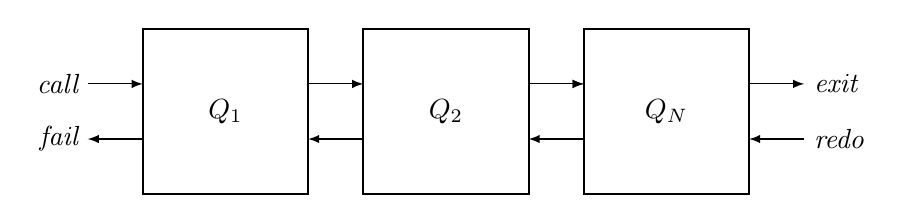
\begin{tikzpicture}[scale=0.7]
            \draw[thick] (0, 0) rectangle (3, 3);

            \draw[-latex] (-1, 2) node[anchor=east] {\it call} -- (0, 2);
            \draw[latex-] (-1, 1) node[anchor=east] {\it fail} -- (0, 1);
            \draw[-latex] (3, 2) -- (4, 2);
            \draw[latex-] (3, 1) -- (4, 1);
            \node at (1.5, 1.5) { $Q_1$ };

            \draw[thick] (4, 0) rectangle (7, 3);
            \draw[-latex] (7, 2) -- (8, 2);
            \draw[latex-] (7, 1) -- (8, 1);
            \node at (5.5, 1.5) { $Q_2$ };

            \draw[thick] (8, 0) rectangle (11, 3);
            \draw[-latex] (7, 2) -- (8, 2);
            \draw[latex-] (12, 2) node[anchor=west] {\it exit} -- (11, 2);
            \draw[-latex] (12, 1) node[anchor=west] {\it redo} -- (11, 1);
            \node at (9.5, 1.5) { $Q_N$ };


        \end{tikzpicture}
    \end{figure}

\end{frame}
